\documentclass{article}
\usepackage{graphicx}
\usepackage[margin=1in]{geometry}
\usepackage{amsmath}
\usepackage{amssymb}
\usepackage{amsthm}
\usepackage{booktabs}
\usepackage{enumitem}
\usepackage{hyperref}
\usepackage{float}
\emergencystretch=3em
\title{Aryan K STAT 37711 PS3}
\author{Aryan Kaushal}
\begin{document}
\maketitle


\section*{Problem 1}

\begin{enumerate}[label=\alph*.]
\item
\begin{enumerate}[label=\roman*.]
\item $Y\in\{0,1,2,\ldots\}$ is a count, and the Poisson is a distribution on exactly the non-negative integers, the standard model for counts of many rare, roughly independent events

It has a single parameter, the rate $\lambda(x)=\mathbb E[Y\mid X=x]>0$, so the model only needs to learn one positive function of $x$; a Normal model with squared error would instead place mass on negative and non-integer values

\item The trees output real numbers, so $f(x)=\sum_j\lambda_jh_j(x)\in\mathbb R$ is unconstrained, while the Poisson rate must satisfy $\lambda(x)>0$; the link $\lambda(x)=e^{f(x)}$ maps $\mathbb R$ onto $\mathbb R_+$, so every value of $f$ gives a valid distribution

It is also the canonical link: $\eta=\log\mathbb E[Y\mid x]$ is the Poisson's natural parameter, so setting $\eta(x)=f(x)$ is the lecture's recipe of letting the predictor be the natural parameter, and it gives the simple loss and gradient below
\end{enumerate}

\item The loss is the negative log-likelihood of $Y\sim\operatorname{Poi}(e^{f(x)})$:
\[L(y,f(x))=-\log\left(\frac{e^{yf(x)}\exp(-e^{f(x)})}{y!}\right)=e^{f(x)}-y\,f(x)+\log(y!)\]

The term $\log(y!)$ does not depend on $f$, so one can equivalently use $L(y,f(x))=e^{f(x)}-yf(x)$, and learning minimizes $\frac{1}{n}\sum_{i=1}^n\left(e^{f(x_i)}-y_if(x_i)\right)$

\item $\dfrac{dL}{df(x)}=e^{f(x)}-y=\lambda(x)-y$

\item Build partial models $f_m=f_{m-1}-\rho_m\hat g_m$, starting from the best constant $f_0=\log\bar y$ (assuming $\bar y>0$)

\textbf{At step $m=1,2,\ldots,M$:}
\begin{enumerate}[label=\arabic*.]
\item Compute the pseudo-outcomes (the gradient at the current model)
\[\gamma_i=\frac{\partial L(y_i,f(x_i))}{\partial f(x_i)}\Big|_{f=f_{m-1}}=e^{f_{m-1}(x_i)}-y_i,\qquad i=1,\ldots,n\]
\item Project the gradient onto trees: fit a regression tree to $\{(x_i,\gamma_i)\}_{i=1}^n$ with squared error,
\[\hat g_m=\operatorname*{argmin}_{h\in\mathcal H}\sum_{i=1}^n(\gamma_i-h(x_i))^2\]
where $\mathcal H$ is regression trees of a fixed maximum depth
\item Choose the step size by line search,
\[\rho_m=\operatorname*{argmin}_\rho\sum_{i=1}^nL\big(y_i,\,f_{m-1}(x_i)-\rho\hat g_m(x_i)\big)\]
or use a fixed learning rate $\rho>0$
\item Update $f_m=f_{m-1}-\rho_m\hat g_m$
\end{enumerate}

In the notation of the problem, $h_m=\hat g_m$ is the $m$th tree and $\lambda_m=-\rho_m$
\end{enumerate}

\section*{Problem 2}
Code at: \url{https://github.com/aryankaushal06/STAT-37711-A26-PSet-Code/blob/main/PS3/p2.py}

\begin{enumerate}[label=\alph*.]
\item The training set $\mathcal D^{\mathrm{train}}$ of size $n$ is used to fit one predictor per hyperparameter setting, giving $\hat f_1,\ldots,\hat f_k$

A test set $\mathcal D^{\mathrm{test}}=\{(x_j,y_j)\}_{j=1}^l$, drawn i.i.d. from $P$ and independent of $\mathcal D^{\mathrm{train}}$, selects $\hat J=\operatorname*{argmin}_{1\leq r\leq k}\hat{\mathcal L}(\hat f_r)$, where $\hat{\mathcal L}(f)=\frac{1}{l}\sum_{j=1}^lL(y_j,f(x_j))$ and $\mathcal L(f)=\mathbb E[L(Y,f(X))]$

Assume the loss is bounded, $0\leq L\leq b$ (for squared error this holds with $b=(y_{\max}-y_{\min})^2$ when $Y\in[y_{\min},y_{\max}]$ and predictions are clipped to that range)

\textbf{Claim:} for any $\delta\in(0,1)$, with probability at least $1-\delta$,
\[\left|\mathcal L(\hat f_{\hat J})-\hat{\mathcal L}(\hat f_{\hat J})\right|\leq b\sqrt{\frac{\log(2k/\delta)}{2l}}=:\varepsilon\]

\textbf{Proof:} Hoeffding's inequality cannot be applied to $\hat f_{\hat J}$ directly, because $\hat J$ depends on the test set, so the losses $L(y_j,\hat f_{\hat J}(x_j))$ are not i.i.d. with mean $\mathcal L(\hat f_{\hat J})$; instead we use a union bound over the $k$ candidates

Condition on $\mathcal D^{\mathrm{train}}$, so that each $\hat f_r$ is a fixed function

Since $\mathcal D^{\mathrm{test}}$ is independent of $\mathcal D^{\mathrm{train}}$, for fixed $r$ the variables $W_j=L(y_j,\hat f_r(x_j))\in[0,b]$ are i.i.d. with mean $\mathcal L(\hat f_r)$, and two-sided Hoeffding gives
\[P\left(\left|\mathcal L(\hat f_r)-\hat{\mathcal L}(\hat f_r)\right|>t\;\middle|\;\mathcal D^{\mathrm{train}}\right)\leq2\exp\left(-\frac{2lt^2}{b^2}\right)\]

The bad event for the selected model is contained in the event that some candidate is bad, so
\[P\left(\left|\mathcal L(\hat f_{\hat J})-\hat{\mathcal L}(\hat f_{\hat J})\right|>t\;\middle|\;\mathcal D^{\mathrm{train}}\right)\leq P\left(\exists r:\left|\mathcal L(\hat f_r)-\hat{\mathcal L}(\hat f_r)\right|>t\;\middle|\;\mathcal D^{\mathrm{train}}\right)\leq2k\exp\left(-\frac{2lt^2}{b^2}\right)\]

The right side does not depend on $\mathcal D^{\mathrm{train}}$, so taking expectations over $\mathcal D^{\mathrm{train}}$ gives the same bound unconditionally; setting $2k\exp(-2lt^2/b^2)=\delta$ gives $t=\varepsilon$ $\qquad\blacksquare$

The bound depends on the test-set size $l$ and on the number of candidate settings $k$ only through $\log k$, and does not depend on $n$; $n$ affects only how good the candidates $\hat f_r$ are

\item If the same test set is used both to select hyperparameters and to report the error, the reported number $\hat{\mathcal L}(\hat f_{\hat J})=\min_r\hat{\mathcal L}(\hat f_r)$ is the minimum of $k$ noisy estimates

Each $\hat{\mathcal L}(\hat f_r)$ alone is unbiased given the training data, but the minimum is not:
\[\mathbb E\left[\min_r\hat{\mathcal L}(\hat f_r)\;\middle|\;\mathcal D^{\mathrm{train}}\right]\leq\min_r\mathbb E\left[\hat{\mathcal L}(\hat f_r)\;\middle|\;\mathcal D^{\mathrm{train}}\right]=\min_r\mathcal L(\hat f_r)\]
so the reported error is optimistically biased as an estimate of the selected model's true risk $\mathcal L(\hat f_{\hat J})\geq\min_r\mathcal L(\hat f_r)$

The more candidates we compare, the more likely one of them has a test error that is low by chance: the bound in (a) controls the gap only while $\log k\ll l$, and when $k$ is large relative to $l$ it becomes vacuous

In effect the test set becomes training data and we overfit to it, and no untouched data remains to estimate the risk of the final model; this is why a separate validation set is used for selection, leaving the test set for one final evaluation

\item Split rows at random into $3428$ training ($70\%$), $490$ validation ($10\%$), and $980$ test ($20\%$) rows

We use KNeighborsRegressor and RandomForestRegressor

KNN predicts the (possibly distance-weighted) average target of the $K$ nearest training points, so I standardize features on the training set and search over $K\in\{1,\ldots,150\}$, weights $\in\{$uniform, distance$\}$, and Minkowski power $p\in\{1,2\}$ (Manhattan or Euclidean distance): $600$ settings

A random forest averages trees fit to bootstrap samples with a random subset of candidate features at each split; I search over n\_estimators $\in\{50,100,200\}$, max\_depth $\in\{\text{None},4,8,12,16,24\}$, min\_samples\_leaf $\in\{1,2,4,8,16\}$, and max\_features (fraction of features tried per split) $\in\{0.2,0.33,0.5,0.75,1.0,\sqrt p\}$: $540$ settings

Both grids exceed the $490$ validation points; each setting is fit on the training set, the one with smallest validation MSE is selected, and only that setting is evaluated on the test set

\begin{table}[H]
\centering
\begin{tabular}{llccc}
\toprule
Model & Selected hyperparameters & Train MSE & Val.\ MSE & Test MSE \\
\midrule
KNN & $K=15$, distance weights, $p=2$ & 0.0000 & 0.4209 & 0.3495 \\
Random forest & 100 trees, no depth limit, leaf $\geq1$, feat.\ $0.33$ & 0.0553 & 0.4010 & \textbf{0.3191} \\
Training mean & --- & --- & 0.8272 & 0.7203 \\
\bottomrule
\end{tabular}
\caption{Selected configurations; the last row predicts the training mean $5.869$ for every point}
\end{table}

The test MSEs are $\boxed{0.3495}$ for KNN and $\boxed{0.3191}$ for the random forest, less than half the baseline's $0.7203$; KNN has zero training error because with distance weights each training point is its own nearest neighbor

\textbf{Validation vs.\ test risk:} By (b), the validation MSE of the selected model is optimistically biased, since it is the minimum over $600$ or $540$ validation errors, while the test MSE, computed once after selection, is an unbiased estimate of the selected model's risk

Here, however, the test MSE is lower than the validation MSE for both models ($0.3495$ against $0.4209$, and $0.3191$ against $0.4010$)

The training-mean baseline, which involves no selection, shows a gap of the same size ($0.7203$ against $0.8272$), so the difference may reflect sampling variability between the $490$ validation and $980$ test points rather than selection; the selection bias is smaller than this variation and cannot be separated from it with a single split
\end{enumerate}

\section*{Problem 3}

Code at: \url{https://github.com/aryankaushal06/STAT-37711-A26-PSet-Code/blob/main/PS3/p3.py}

Each dataset has $500$ rows, a binary label in the first column, and $5$ features

We fit GradientBoostingClassifier (logistic loss, learning rate $0.1$, depth-$3$ trees: the scikit-learn defaults) with $M\in\{1,10,100,300,1000\}$ trees

Since $n=500$ is small, a single test split is noisy, so I repeat a stratified $70/30$ train/test split over $20$ seeds and report mean $\pm$ standard deviation of the classification error; for each split one $1000$-tree fit gives every smaller model through staged\_predict, since the first $M$ trees of a boosted model are the $M$-tree model

\begin{table}[H]
\centering
\begin{tabular}{rcccc}
\toprule
& \multicolumn{2}{c}{dset0} & \multicolumn{2}{c}{dset1} \\
\cmidrule(lr){2-3}\cmidrule(lr){4-5}
$M$ & Train err & Test err & Train err & Test err \\
\midrule
1 & 0.426 & $0.427\pm0.000$ & 0.281 & $0.319\pm0.077$ \\
10 & 0.150 & $0.275\pm0.031$ & 0.114 & $0.206\pm0.027$ \\
100 & 0.004 & $0.180\pm0.026$ & 0.010 & $\mathbf{0.186}\pm0.030$ \\
300 & 0.000 & $\mathbf{0.177}\pm0.028$ & 0.000 & $0.196\pm0.028$ \\
1000 & 0.000 & $0.180\pm0.027$ & 0.000 & $0.200\pm0.027$ \\
\bottomrule
\end{tabular}
\caption{Gradient boosting classification error, means over $20$ splits}
\end{table}

\begin{figure}[H]\centering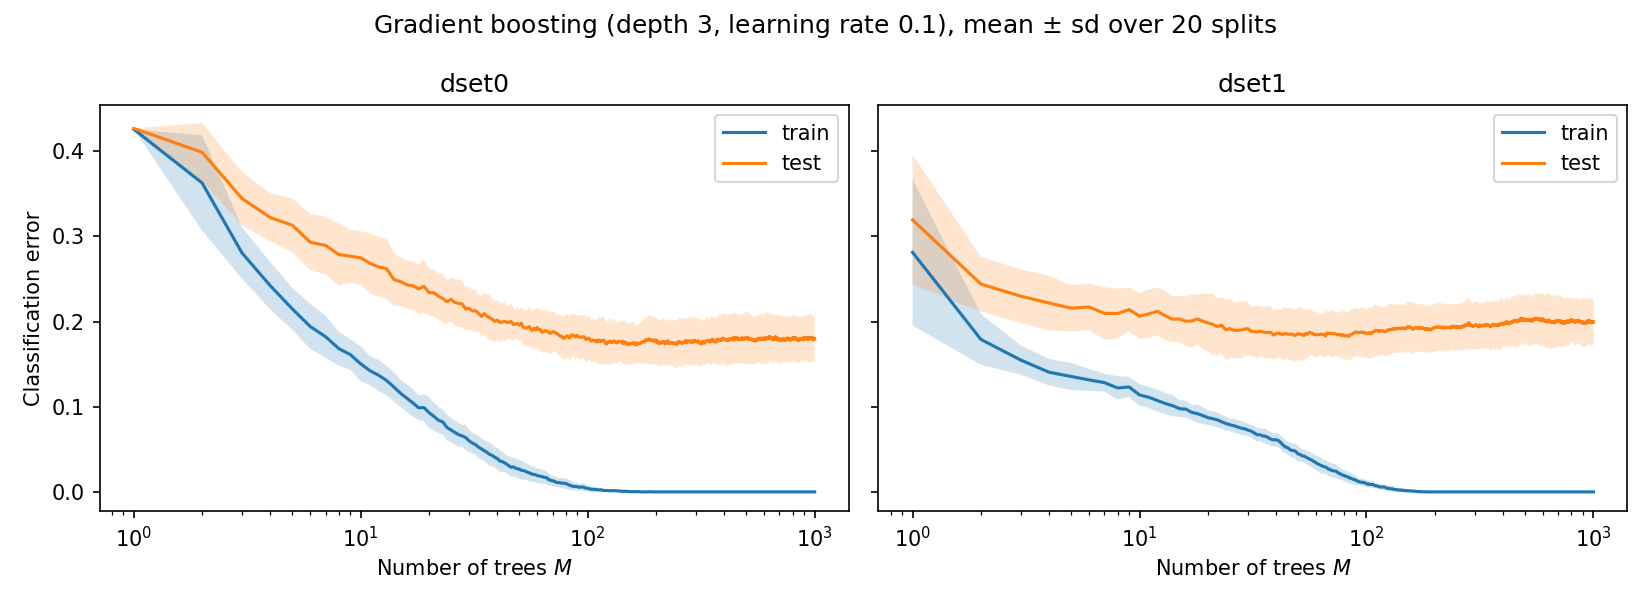
\includegraphics[width=\textwidth]{figures/p3_error_curves.png}\caption{Training and test error against the number of trees, mean $\pm$ sd over $20$ splits}\end{figure}

\begin{enumerate}[label=\alph*.]
\item \textbf{dset0:} Test error falls from $0.427$ (one tree, which only predicts the majority class) to $0.275$ at $M=10$ and $0.180$ at $M=100$, and then stays flat: $0.177$ at $M=300$ and $0.180$ at $M=1000$

Training error is $0$ by $M=300$, yet adding $700$ more trees does not increase the test error

As in the MNIST example from lecture, additional boosting rounds increase model complexity but do not cause overfitting in classification error

\item \textbf{dset1:} Test error is lowest near $M=100$ ($0.186$) and then rises to $0.196$ at $M=300$ and $0.200$ at $M=1000$, while training error is $0$

This suggests mild overfitting: once training error reaches $0$, additional trees slightly worsen test error, as in the heart-disease example from lecture

\item One possible explanation is that dset0 has approximately separable classes (the label is close to a deterministic function of the features), while dset1 has greater label noise or class overlap

On separable data, continued boosting keeps increasing the margins $y_is(x_i)$ of the training points, and larger margins give a better generalization bound, so test error need not rise after training error reaches $0$

With noisy labels, the training points can only be separated by fitting the noise, so additional trees reduce training error while worsening generalization

This is consistent with the different behavior observed in (a) and (b), and suggests choosing the number of trees on validation data (early stopping) when the labels may be noisy
\end{enumerate}
\end{document}
